\documentclass[../main.tex]{subfiles}
\hbadness=1000000
\vbadness=1000000
\begin{document}

\section{Methods}

\subsection{Network model}
The hippocampal network model is composed of 1600 five-compartment pyramidal cells, along with 200 single-compartment PV basket interneurons, 60 single-compartment OLM interneurons, and an additional 70 single-compartment non-basket CCK interneurons. 
Notably, these interneurons primarily exhibit local inhibition. 
To maintain consistency between the CA1 and CA3 subregions, the cell numnbers were determined to preserve the relative proportions between pyramidal cells and interneurons \citep{bezaire_interneuronal_2016,gandolfi_full-scale_2023}.
Specifically, the CA3 region encompasses 800 pyramidal cells, 100 PV basket cells, and 30 OLM cells.
\begin{figure}[!htb]
    \centering
    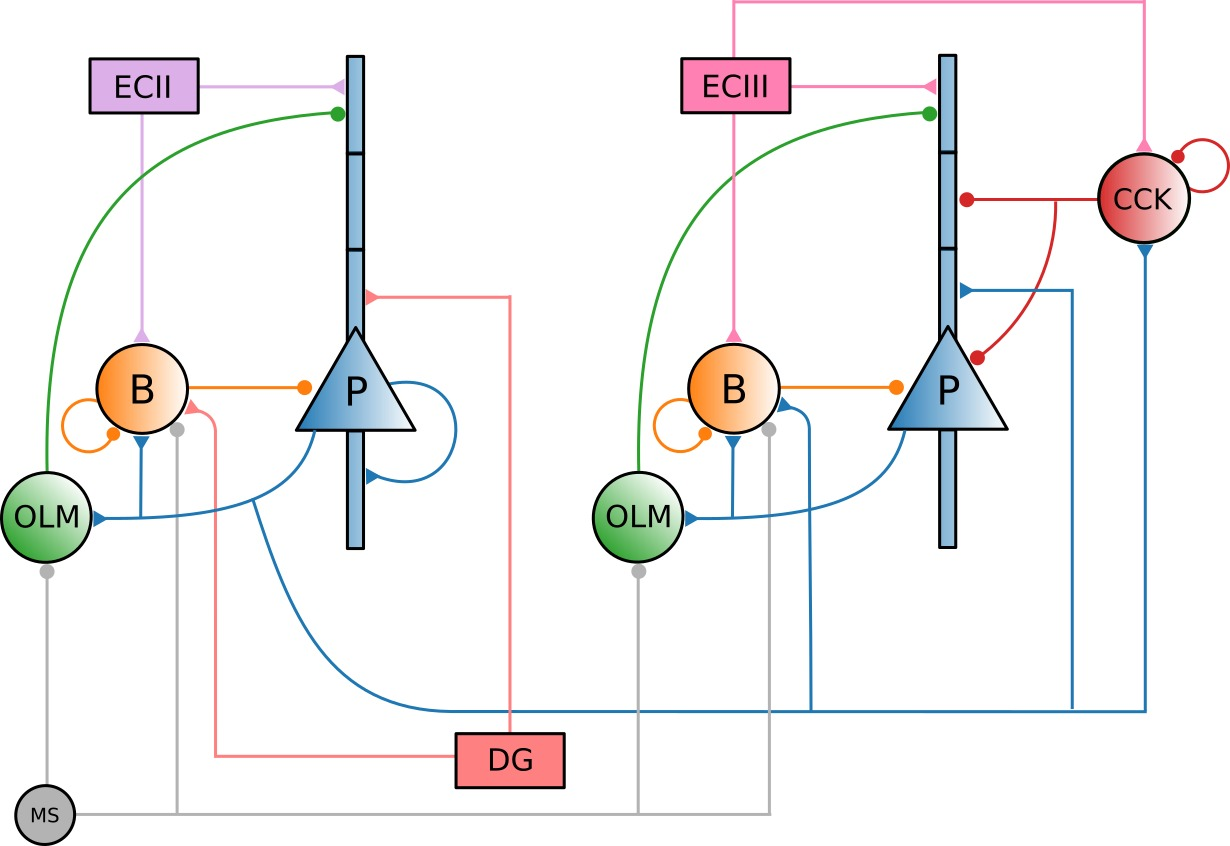
\includegraphics[width=\textwidth]{chapter4/figures/hippocampus_network.jpeg}
    \caption{\textbf{Schmeatic representation of the hippocampal network model}.
    CA3 subfield is formed by excitatory pyramidal cells (P) and inhibitory basket (B) and OLM cells.
    It receives external projections from the medial septum (MS), enthorrinal cortex layer II (ECII) and the dendate gyrus (DG).
    CA1 subfiled is formed by excitatory pyramidal cells (P) and inhibitory basket (B), OLM and CCK cells.
    It receives external projection from the medial septum (MS) and enthorrinal cortex layer III (ECIII),
    Circles and triangles indicate inhibition and excitation, respectively.}
    \label{fig:network-model}
\end{figure}
Similarly, the CA1 region mirrors these counts while accommodating an additional 70 non-basket CCK cells, all aligned with established proportions.
Figure \ref{fig:network-model} illustrates a schematic representation of the network model, delineating the intricate web of connections among cells and their associated external inputs.
The model for the CA3 region draws inspiration from prior studies \citep{neymotin_ketamine_2011,neymotin_ih_2013}, serving as a foundational framework.
Meanwhile, the CA1 region model closely resembles the architecture of CA3 but incorporates notable distinctions.
These distinctions include the absence of self-excitation among pyramidal neurons, the integration of an additional interneuron subtype, the non-basket CCK cells, and the inclusion of external inputs projected from extrahippocampal regions, specifically the inputs from the Entorhinal Cortex layer III (ECIII).

Implemented within the Python-Neuron environment \citep{hines_neuron_2009}, the multicompartmental model of pyramidal cells necessitates precise dimensioning for each compartment.
Specific sizes are assigned to individual compartments, delineated by the cylinder's length and base radius, as detailed in Table \ref{table:pyr-parameters}.
Conversely, single-compartment interneurons are uniformly set at a size of 100 $\mu$m$^2$, a measure enabling a consistent current density - point current equivalence of 1 $\mu$A/cm$^2$ = 1 $p$A. 
This standardization is crucial, considering Neuron's configuration, where synaptic recordings are denoted in $p$A, while parameters must be articulated in density units.
Such standardization adheres to widely recommended conventions within the Neuron community, addressing issues pertinent to data coherence and compatibility among users and developers.

For the sake of brevity and clarity in our model's nomenclature, the PV basket cells will henceforth be referred to as basket cells, and the non-basket CCK cells as CCK cells.
\subsubsection{Basket cells}
Basket cells are neurons of one compartment whose dynamics are described by the Wang and Buzsaki interneuron model \citep{neymotin_ketamine_2011,neymotin_ih_2013,Tort2007,Wang1996}.
The membrane potential $v$ dynamics is given by:
\begin{equation}
    C\displaystyle\frac{dv}{dt} = I_{\text{app}}-I_{\text{Na}} - I_{\text{K}} - I_{\text{L}} - I_{\text{syn}},
    \label{eq:basket-dynamics}
\end{equation}
where $I_{\text{app}}$ is the applied current, $I_{\text{syn}}$ is the total synaptic current, $I_{\text{L}}$ is the leak current, $I_{\text{Na}}$ is the transient sodium current, and $I_{\text{K}}$ is the delayed rectifier potassium current. 
The dynamics of each current is described by:
\begin{enumerate}
    \item \underline{Leak current}. 
        \begin{equation}
            I_{\text{L}} = g_{\text{L}}(v-E_{\text{L}}).
            \label{eq:basket-leak-current}
        \end{equation}
    \item \underline{Transient sodium current}. 
        \begin{equation}
        \begin{aligned}
            &\hspace{-2.8cm}I_{\text{Na}} = g_{\text{Na}}m_{\infty}^3h(v-E_{\text{Na}}),  \\
            & \\
        \begin{aligned}
            m_\infty &= \displaystyle\frac{\alpha_m}{\alpha_m+\beta_m}, \\
            \alpha_m(v) &= \displaystyle\frac{-0.1(v+35)}{\exp{\Big(-0.1(v+35)\Big)}-1},\\ %\hspace{0.2cm}
            \beta_m(v) &= 4\exp{-\bigg(\displaystyle\frac{v+60}{18} \bigg)}, \\
        \end{aligned}
        &
        \begin{aligned}
            \displaystyle\frac{dh}{dt} &= \phi\big(\alpha_h(1-h)-\beta_hh\big),\\
            \alpha_h(v) &= 0.07\exp{\bigg(-\displaystyle\frac{v+56}{20} \bigg)},\\ %\hspace{0.2cm}
            \beta_h(v) &= \Big(\exp{\big(-0.1(v+28)\big)}+1\Big)^{-1}.
        \end{aligned}
        \end{aligned}
        \label{eq:basket-sodium-current}
        \end{equation}
    \item \underline{Delayed rectifier potassium current}.
        \begin{equation}
        \begin{aligned}
            I_{\text{K}} &= g_{\text{K}}n^4(v-E_{\text{K}}), \\
            \displaystyle\frac{dn}{dt} &= \phi\big(\alpha_n(1-n)-\beta_nn\big),\\
            \alpha_n(v) &= \displaystyle\frac{-0.01(v+34)}{\exp{\big(-0.1(v+34)\big)}-1},\\% \hspace{0.2cm}
            \beta_n(v) &= 0.125\exp{\bigg(-\displaystyle\frac{v+44}{80} \bigg)}.
            \label{eq:basket-potassium-current}
        \end{aligned}
        \end{equation}
\end{enumerate}
All the values of the parameters involved in equations \eqref{eq:basket-dynamics}-\eqref{eq:basket-sodium-current} are shown in Table \ref{table:basket-parameters}.
\begin{table}[htb]
\def\arraystretch{1.4}%  1 is the default, change whatever you need
\caption{Parameters of the basket cell model.}
\begin{center}
\begin{tabular}{|c|c|c|c|}
    \hline
    Ionic current & Reversal potential & Conductance & $\phi$ \\ \hline
    Leak (L)      & $E_{\text{L}}$ = -65 $mv$ & $g_{\text{L}}$  = 0.1 $mS/cm^2$ & -\\ \hline
    Sodium (Na)   & $E_{\text{Na}}$ = 55 $mv$ & $g_{\text{Na}}$ = 35 $mS/cm^2$  & $\phi$ = 5\\ \hline
    Potassium (K) & $E_{\text{K}}$ = -90 $mv$ & $g_{\text{K}}$  = 9 $mS/cm^2$   & $\phi$ = 5\\ \hline
    \multicolumn{4}{|c|}{Other parameters}\\ \hline
    Capacitance      &  \multicolumn{3}{c|}{$C$ = 1 $\mu F/cm^2$} \\ \hline
    Applied current  &  \multicolumn{3}{c|}{$I_{\text{app}}$ = 0 $\mu A/cm^2$}\\
    \hline
\end{tabular}
\label{table:basket-parameters}
\end{center}
\end{table}
%%%%%%%%%%%%%%%%%%%%%%%%%%%%%%%%%%%%%%%%%%%%%%%%%%%%%%%%%%%%%%%%%%%%%%%%%
%% OLM cells
%%%%%%%%%%%%%%%%%%%%%%%%%%%%%%%%%%%%%%%%%%%%%%%%%%%%%%%%%%%%%%%%%%%%%%%%%
\subsubsection{OLM cells.}
OLM cells are one-compartment neurons whose dynamics are described by 
\citep{neymotin_ketamine_2011,neymotin_ih_2013,Tort2007}:
\begin{equation}
    C\displaystyle\frac{dv}{dt} = I_{\text{app}}-I_{\text{Na}} - I_{\text{K}} - I_{\text{L}} -I_{\text{h}} -I_{\text{A}} -I_{\text{syn}},
    \label{eq:olm-dynamics}
\end{equation}
where $v$ is the membrane potential, $I_{\text{app}}$ is the external applied current and $I_{\text{K}}$, $I_{\text{L}}$, $I_{\text{h}}$, $I_{\text{A}}$ and $I_{\text{syn}}$ are the leak, the transient sodium, the delayed rectifier potassium, the hyperpolarization-activated mixed cation and A currents, respectively.
The dynamics of each current is described by:
\begin{enumerate}
    \item \underline{Leak}, \underline{transient sodium} and \underline{delayed rectifier potassium currents} are also described by equations \eqref{eq:basket-leak-current}, \eqref{eq:basket-sodium-current} and \eqref{eq:basket-potassium-current}, respectively.
    The same equations for to basket cells.
    \item \underline{Hiperpolarization-activated current}.
        \begin{equation}
        \begin{aligned}
            I_{\text{h}} &= g_{\text{h}} q(v-E_{\text{h}}), \\
            \displaystyle\frac{dq}{dt} &= \displaystyle\frac{q_{\infty}-q}{\tau_q}, \\
            q_{\infty}(v) &= \Bigg[1+\exp{\bigg( \frac{v+80}{10}
            \bigg)}\Bigg]^{-1}, \\
            \tau_q(v) &= 5+200\Bigg[ \exp{\bigg( \displaystyle\frac{v+70}{20}\bigg)}+\exp{\bigg(-\displaystyle\frac{v+70}{20}\bigg)}\Bigg]^{-1}.
            \label{eq:olm-hiperpolarization-current}
        \end{aligned}
        \end{equation}
    % \item \underline{Calcium concentration dynamics}.
    %     \begin{equation}
    %         \displaystyle\frac{[\text{Ca}^{2+}]_{i}}{dt} = -\alpha I_{\text{Ca}}-\displaystyle\frac{[\text{Ca}^{2+}]_{i}}{\tau_{\text{Ca}}}, \\
    %         \label{eq:olm-calcium-current}
    %     \end{equation}
    \item \underline{Calcium current}. 
        \begin{equation}
        \begin{aligned}
        I_{\text{Ca}} &= g_{\text{Ca}}m_\infty^2(v-E_{\text{Ca}}), \\
        m_\infty &= \Bigg[ 1+\exp{ \bigg( -\displaystyle\frac{v+20}{9} \bigg)} \Bigg]^{-1}.
        \label{eq:olm-calcium-current-2}
        \end{aligned}
        \end{equation}
    \clearpage
     \item \underline{Calcium-activated potassium current}.
        \begin{equation}
        \begin{aligned}
            I_{\text{KCa}} &= g_{\text{KCa}}\displaystyle\frac{[\text{Ca}^{2+}]_{i}}{[\text{Ca}^{2+}]_{i}+k_d}(v-E_{\text{K}}),\\
            \displaystyle\frac{d[\text{Ca}^{2+}]_{i}}{dt} &= -\alpha I_{\text{Ca}}-\displaystyle\frac{[\text{Ca}^{2+}]_{i}}{\tau_{\text{Ca}}}, \\
        \end{aligned}
        \label{eq:olm-potassium-current}
        \end{equation}
        where $[\text{Ca}^{2+}]_{i}$ is the calcium concentration.
\end{enumerate}
All the values of the parameters involved in equations \eqref{eq:olm-dynamics} - \eqref{eq:olm-calcium-current-2} are shown in Table \ref{table:olm_parameters}.
\begin{table}[htb]
\def\arraystretch{1.4}
\caption{Parameters of the OLM cell model.}
\begin{center}
\begin{tabular}{|c|c|c|c|}
    \hline
    Ionic current & Reversal potential & Conductance & $\phi$ \\ \hline
    Leak (L)      & $E_{\text{L}}$ = -65 $mv$ & $g_{\text{L}}$  = 0.1 $mS/cm^2$ & -\\ \hline
    Sodium (Na)   & $E_{\text{Na}}$ = 55 $mv$ & $g_{\text{Na}}$ = 35 $mS/cm^2$  & $\phi$ = 5\\ \hline
    Potassium (K) & $E_{\text{K}}$ = -90 $mv$ & $g_{\text{K}}$  = 9 $mS/cm^2$   & $\phi$ = 5\\ \hline
    Calcium (Ca)  & $E_{\text{Ca}}$ = 120 $mv$ & $g_{\text{Ca}}$ = 1 $mS/cm^2$  & - \\ 
    \hline
    \multicolumn{4}{|c|}{Other parameters}\\ \hline
    Calcium dynamics &\multicolumn{3}{c|}{$\alpha$ = 2 $cm^2mM/(mA ms)$, $\tau_{\text{Ca}}$ = 80 $ms$, $k_d$ = 30 $mM$} \\
    \hline
    Capacitance      &  \multicolumn{3}{c|}{$C$ = 1$\mu F/cm^2$} \\ \hline
    Applied current  &  \multicolumn{3}{c|}{$I_{\text{app}}$ = -25$\mu A/cm^2$}\\
    \hline
\end{tabular}
\label{table:olm_parameters}
\end{center}
\end{table}

%%%%%%%%%%%%%%%%%%%%%%%%%%%%%%%%%%%%%%%%%%%%
%% Pyramidal cells
%%%%%%%%%%%%%%%%%%%%%%%%%%%%%%%%%%%%%%%%%%%%
\subsubsection{Pyramidal cells}
Pyramidal cells are five-compartment neurons, the soma and four dendritic compartments: basal dendrites, Bdend, and apical dendrites 1, 2 and 3, Adend1, Adend2 and Adend3, respectively.
The dimensions of each compartment are described in Table \ref{table:pyr-parameters}.
The time dependence of the membrane potential of the $k$-th compartment is described by \citep{neymotin_ketamine_2011,neymotin_ih_2013,Tort2007,}:
\begin{equation}
    C_k\displaystyle\frac{dv_k}{dt} = I_{\text{app},k}-I_{\text{Na},k} - I_{\text{K},k} - I_{\text{L},k} -I_{\text{h},k} -I_{\text{syn}} + I_{\text{conn},k}.
    \label{eq:pyr-dynamics}
\end{equation}
where $v$ is the membrane potential, $I_{\text{app}}$ is the external applied current and $I_\text{Na}$, $I_{\text{K}}$, $I_{\text{L}}$, $I_{\text{h}}$,  and $I_{\text{syn}}$ are the transient sodium, the delayed rectifier potassium, the leak, the hyperpolarization-activated mixed cation and the synaptic currents, respectively. 
$I_{\text{conn},k}$ is the intradendritic current that compartment $k$ receives from its colindant compartments $k-1$ and $k+1$.
It is defined as follows:
\begin{equation}
    I_{\text{conn},k} = g_{k,k+1}(v_{k+1}-v_k) + g_{k,k-1}(v_{k-1}-v_k),
    \label{eq:dendritic-current}
\end{equation}
where the coupling conductance is given by:
\begin{equation}
    g_{k,j} = \displaystyle\frac{r_k r_j^2}{R_aL_k(L_kr_j^2 + L_jr_k^2)}
    \label{eq:dendritic-coupling}
\end{equation}
The description of each current is given by:
\begin{enumerate}
    \item \underline{Leak current}.
        \begin{equation}
            I_{\text{L},k} = g_{\text{L},k}(v_k - E_{\text{L},k}). 
            \label{eq:pyr-leak-current}
        \end{equation}      
    \item \underline{Transient sodium current}. 
        \begin{equation}
        \begin{aligned}
            &\hspace{-2.8cm}I_{\text{Na},k} = g_{\text{Na},k} m^3hi(v_k-E_{\text{Na},k}), \\
        &\hspace{-2.8cm}\displaystyle\frac{dx}{dt} = \displaystyle\frac{x_\infty-x}{\tau_x}, \hspace{0.2cm} x = \{ m,h,i\},\\
        & \\
        \begin{aligned}
            m_\infty &= \displaystyle\frac{\alpha_m}{\alpha_m+\beta_m},\\% \hspace{0.2cm}
            \tau_m &= \max \bigg(0.2, \displaystyle\frac{0.5}{\alpha_m+\beta_m}\bigg),\\
            \alpha_m(v_k) &= \displaystyle\frac{0.4(v_k+30)}{1-\exp{\Big(-\frac{v_k+30}{7.2}\Big)}},\\ %\hspace{0.2cm}
            \beta_m(v_k)   &= \displaystyle\frac{0.124(v_k+30)}{\exp{\Big(\frac{v_k+30}{7.2}\Big)-1}}, \\
            h_\infty(v_k) &= \Bigg[1+\exp{\bigg(\frac{v_k+50}{4} \bigg)}\Bigg]^{-1}\\ %, \hspace{0.2cm}
            \tau_{h} &= \max\bigg(0.5, \displaystyle\frac{0.5}{\alpha_h+\beta_h}\bigg), \\
        \end{aligned}
        & 
        \begin{aligned}
            \alpha_h(v_k) &= \displaystyle\frac{0.03(v_k+45)}{1-\exp{\Big(\frac{v_k+45}{1.5}\Big)}},\\ % \hspace{0.2cm}
            \beta_h(v_k)  &= \displaystyle\frac{0.01(v_k+45)}{\exp{\Big( \frac{v_k + 45}{1.5}\Big)}-1}, \\
            i_\infty(v_k) &= \displaystyle\frac{1+b_k\exp{\Big(\frac{v_k+60}{2} \Big)}}{1+\exp{\Big( \frac{v_k+60}{2}\Big)}}, \\ % \hspace{0.2cm}
            \tau_i &= \max\bigg(10, \displaystyle\frac{30000\beta_i}{1+\alpha_i} \bigg), \\
            \alpha_i(v_k) &= \exp{\big( 0.45(v_k+66)\big)},\\ % \hspace{0.2cm} 
            \beta_i(v_k) &= \exp{\big(0.09(v_k+66)\big)}.
            \label{eq:pyr-sodium-current}
        \end{aligned}
        \end{aligned}
        \end{equation}
    \item \underline{Delayed rectifier potassium current}.
        \begin{equation}
        \begin{aligned}
            I_{\text{K},k} &= g_{\text{K},k}n^4(v_k-E_{\text{K},k}), \\        
            n_\infty &= \displaystyle\frac{1}{1+\alpha_n}, \\ %\hspace{0.2cm} 
            \tau_n &= \max \Big(2, \displaystyle\frac{50\beta_n}{1+\alpha_n}\Big), \\
            \alpha_n(v_k) &= \exp{\big(-0.11(v_k-13)\big)}, \\% \hspace{0.2cm} 
            \beta_n(v_k)  &= \exp{\big(-0.09(v_k-13)\big)}.
            \label{eq:pyr-potassium-current}
        \end{aligned}
        \end{equation}
    \item \underline{Hyperpolarization-activated current}.
        \begin{equation}
        \begin{aligned}
            I_{\text{h},k} &= g_{\text{h},k}r(v_k-E_{\text{h},k}), \\
            \displaystyle\frac{dr}{dt} &= \displaystyle\frac{r_\infty-r}{\tau_r},\\
            r_{\infty,\text{HCN2}}(v_k) &= \Bigg[1+\exp{\Bigg( \displaystyle\frac{v_k-v_{50,k}}{10.5}\Bigg)} \Bigg]^{-1} \\
            \tau_{r,\text{HCN2}}(v_k) &= \Big( \exp{\big(-14.59-0.086v_k\big)} +\\ 
            \quad &\quad\quad\exp{\big(-1.87+0.0701v_k\big)}\Big)^{-1},  \\
            r_{\infty,\text{HCN1}}(v_k) &= \Bigg[1+\exp{( 0.151(v_k-v_{50,k})} \Bigg]^{-1}, \\
            \tau_{r,\text{HCN1}}(v_k) &= \displaystyle\frac{\exp{\big(0.033(v_k+75)\big)}}{0.011\Big(1+\exp{\big(0.083(v_k+75) \big)}\Big)}.
            \label{eq:pyr-hyperpolarization-current}
        \end{aligned}
        \end{equation}
        \clearpage
    \item \underline{Potassium A-type current}. 
        \begin{equation}
        \begin{aligned}
            I_{\text{A},k} &= g_{\text{A},k} ab(v_k-E_{\text{A},k}), \\
            \displaystyle\frac{dx}{dt} &= \displaystyle\frac{x_\infty-x}{\tau_x}, \hspace{0.2cm} x = \{a,b\}, \\
            a_\infty &= \displaystyle\frac{1}{1+\alpha_a},\\ %\hspace{0.2cm}
            \tau_a &= \max\Bigg(0.1, \displaystyle\frac{c_k\beta_a}{1+\alpha_m} \Bigg), \\
            \alpha_a(v_k) &= \exp{\Bigg[ -0.038\Bigg(d_k + \bigg(1+\displaystyle\frac{\exp{(v_k+40)}}{5}\bigg)^{-1}\Bigg)(v_k-e_k)\Bigg]}, \\
            \beta_a(v_k) &= \exp{\Bigg[ -0.038\Bigg(f_k + \bigg(1+\displaystyle\frac{\exp{(v_k+40)}}{5}\bigg)^{-1}\Bigg)(v_k-e_k)\Bigg]}, \\
            b_\infty(v_k) &= \displaystyle\frac{1}{1+\exp{\Big(0.11(v_k+56)\Big)}}, \\
            \tau_b(v_k) &= \max\big(2,0.26(v_k+50)\big).
            \label{eq:pyr-A-current}
        \end{aligned}
        \end{equation}
        where $a$ and $b$ are the activation and inactivation variables, respectively.
\end{enumerate}
All the values of the parameters involved in equations \eqref{eq:pyr-dynamics} - \eqref{eq:pyr-A-current} are shown in Table \ref{table:pyr-parameters}.
\begin{table}[htb]
\caption{Parameters of CA3 (CA1) Pyramidal cell model.}
\begin{center}
\def\arraystretch{1.3}%  1 is the default, change whatever you need
\begin{tabular}{|c|c|c|c|c|c|c|}
\hline
 Ionic currents &Parameters & Bdend & Soma & Adend1 & Adend2 & Adend3 \\
 \hline
  Leak (L)     & $g_{\text{h}}$ [$mS/cm^2$] & 0.1 & 0.1 & 0.2 & 0.4 & 0.7 \\  \hline
  \multirow{2}{*}{Sodium (Na)}  & $g_{\text{Na}}$ [$mS/cm^2$]& 32  & 32  & 32  & 32  & 32  \\ \cline{2-7}
                                  & $b$ & 1 & 0.8 & 0.5 & 0.5 & 0.5 \\ \hline
  Potassium (K) & $g_{\text{k}}$ [$mS/cm^2$] & 10  & 10  & 10  & 10  & 10  \\  \hline
  
  \multirow{5}{2cm}{Potassium type-A (A)} & $g_{\text{A}}$ [$mS/cm^2$] & 48  & 48  & 72  & 120 & 200  \\ \cline{2-7} 
                                     & $v_{50}$ [$mv$] & -82 & -82 & -82 & -90 (-82) & -90 (-82) \\ \cline{2-7}
                                     & $c$ & 4 &  4  & 4   & 2 & 2                               \\ \cline{2-7}
                                     & $d$ & 1.5 & 1.5 & 1.5 & 1.8 & 1.8                         \\ \cline{2-7}
                                     & $e$ [$mv$] & 11 & 11  & 11 & 11 & 11                      \\ \cline{2-7} 
                                     & $f$ & 0.825 & 0.825 & 0.825 & 0.825 & 0.825 \\ 
  \hline
  \hline
  Applied current & $I_{\text{app}}$ [$mA/cm^2$] & 0 & 25 & 0 & 0 & 0 \\\hline
  Capacitance     & $C$ [$\mu F/cm^2$]           & 1 & 1  & 1 & 1 & 1 \\ \hline
  Length & l [$\mu m$] & 200 & 20 & 150 & 150 & 150 \\ \hline
  Radius & r [$\mu m$] & 10  & 1  & 1   & 1   & 1   \\ \hline
\end{tabular}
\label{table:pyr-parameters}
\end{center}
\end{table} 
%%%%%%%%%%%%%%%%%%%%%%%%%%%%%%%%%%%%%%%%%%%%%%%%%%%%%%%%%%%%%%%%%%%%%%%%%
%% CCK cells
%%%%%%%%%%%%%%%%%%%%%%%%%%%%%%%%%%%%%%%%%%%%%%%%%%%%%%%%%%%%%%%%%%%%%%%%%
\subsubsection{CCK cell}
Non-basket CCK cells consisted in a monocompartment neurons obtained from a dimension reduction of a complex neuron model of 17 compartments \citep{bilash_lateral_2023}.
For this dimensional reduction, all dendrites initially present in the model were removed and the soma area was fixed at 100 $\mu$m$^2$, similar to other interneurons, in order to maintain equivalence in Neuron between point current and current density.
Subsequently, optimizations were performed on the leak, sodium, and potassium conductances using the least squares method.
To achieve this, we defined a function whose minimization provided the optimal values for these conductances, ensuring that the neuron's response to three different step currents would be as similar as possible. In other words, the aim was for the reduced version to elicit the same number of action potentials, while ensuring the first spike's response time was as closely aligned as feasible.

The membrane potential $v$ of the soma of CCK cells is described by \citep{bilash_lateral_2023,cutsuridis_hippocampal_2018,aradi_role_1999}:
\begin{equation}
 C\displaystyle\frac{dv}{dt} = I_{\text{app}}-I_{\text{Na}} - I_{\text{K}} - I_{\text{L}} - I_{\text{h}} - I_{\text{K-A}}- I_{\text{Ca-K}}- I_{\text{sCa-K}}-I_{\text{N-Ca}}-I_{\text{L-Ca}}-I_{\text{syn}},
    \label{eq:cck-dynamics}
\end{equation}
where, $I_\text{app}$ is the external applied current, $I_\text{Na}$ is the transient sodium current, $I_\text{K}$ is the delayed rectifier potassium current, $I_\text{L}$ is the leak current, $I_\text{h}$ is the hyperpolarization-activated channel-h current, $I_\text{K-A}$ is the Borg-Gragam type generic K-A channel current, $I_\text{N-Ca}$ is N-type calcium channel current, $I_\text{L-Ca}$ is the L-type calcium channel current current, $I_\text{Ca-K}$ is the calcium-activated potassium current, $I_\text{sCa-K}$ is the slow calcium-dependant potassium current, and $I_\text{syn}$ is the synaptic current.
\begin{itemize}
    \item \underline{Leak current}.
        \begin{equation}
            I_\text{L} = g_\text{L}(v-E_\text{L})
            \label{eq:cck-leak-current}
        \end{equation}
    \item \underline{Sodium current}: 
        \begin{equation}
        \begin{aligned}
            &\hspace{-2.8cm}I_{\text{Na}} = g_{\text{Na}}m^3h(v-E_{\text{Na}}), \\
    &\hspace{-2.8cm}\displaystyle\frac{dx}{dt} = \alpha_x(1-x)-\beta_xx, \hspace{0.2cm} x =\{m,h\},\\
            & \\
        \begin{aligned}
            \alpha_m(v) &= \displaystyle\frac{-0.3(v+31)}{\exp{\Big(-\frac{v+31}{5}\Big)-1}},\hspace{3mm}\\%\hspace{0.2cm},
            \beta_m(v) &= \displaystyle\frac{0.3(v+3)}{\exp\Big( \frac{v+3}{5}\Big)-1},\\ 
        \end{aligned}
        &
        \begin{aligned}
            \alpha_h(v) &= 0.23\exp{\bigg(-\displaystyle\frac{v+53}{10} \bigg)},\\ %\hspace{0.2cm}
            \beta_h(v) &= \displaystyle\frac{3.33}{1+\exp{\Big(-\frac{v+0.5}{5}\Big)}}.
        \end{aligned}
        \end{aligned}
        \label{eq:cck-sodium-current}
        \end{equation}
        
    \item \underline{Potassium current}: 
        \begin{equation}
        \begin{aligned}
            I_\text{K} &= g_\text{K}n^4(v-E_\text{K}),\\
            \displaystyle\frac{dn}{dt} &= \alpha_n(1-n)-\beta_nn,\\
            \alpha_n(v) &= \displaystyle\frac{-0.07(v-24)}{\exp{\Big(-\frac{v-24}{6}\Big)}-1}, \\ %\hspace{0.2cm}
            \beta_h(v) & = 0.264\exp{\bigg(-\displaystyle\frac{v+1}{40}\bigg)}.
            \label{eq:cck-potassium-current}
        \end{aligned}
        \end{equation}
    \item \underline{Hyperpolarization-activated channel-h current}. 
        \begin{equation}
        \begin{aligned}
            I_{\text{h}} &= g_{\text{h}}r(v-E_{\text{h}}),\\
            \displaystyle\frac{dr}{dt} &= \displaystyle\frac{r_\infty-r}{\tau_r}, \\
            r_\infty &= \Bigg[ 1+\exp{ \bigg( \displaystyle\frac{v+100}{10} \bigg) }\Bigg]^{-1},\\
            \tau_r &= 20 + 0.01\bigg(\exp{(-17.9-0.116v)} + \exp{(-1.84+0.09v)} \bigg)^{-1}.\\
            \label{eq:cck-hyperpolarization-current}
        \end{aligned}
        \end{equation}
    \clearpage
    \item \underline{Borg-Graham type generic K-A channel}.
        \begin{equation}
        \begin{aligned}
            &\hspace{-2.8cm}I_{\text{K-A}} = g_{\text{K-A}}nl(v-E_{\text{K}}), \\
            &\hspace{-2.8cm}\displaystyle\frac{dx}{dt} = \displaystyle\frac{x_{\infty}-x}{\tau_x}, \hspace{0.2cm} x = \{n,l\},\\
            &\hspace{-2.8cm}x_\infty = \displaystyle\frac{1}{1+\alpha_x},\\% \hspace{0.2cm}
            &\hspace{-2.8cm}\tau_x = \displaystyle\frac{3^{-0.1(T-303.16)}\beta_x}{a_{0,x}(1+\alpha_x)},\\
        & \\
        \begin{aligned}
            \alpha_n(v) &= \exp{\bigg( -289.44\displaystyle\frac{v+33.6}{RT}  \bigg)},\\
            \beta_n(v)  &= \exp{\bigg( -173.664\displaystyle\frac{v+33.6}{RT} \bigg)},\hspace{3mm}\\
        \end{aligned}
        &
        \begin{aligned}
            \alpha_l(v) &= \exp{\bigg( 385.92\displaystyle\frac{v+83}{RT}    \bigg)},\\
            \beta_l(v)  &= \exp{\bigg( 385.92\displaystyle\frac{v+83}{RT}    \bigg)}. \\
        \end{aligned}
        \end{aligned}
        \label{eq:cck-KA-current}
        \end{equation}
    \item \underline{Calcium-activated potassium current}.
        \begin{equation}
        \begin{aligned}
            I_{\text{Ca-K}} &= g_{\text{Ca-K}}q^2(v-E_{\text{K}}), \\
            \displaystyle\frac{dq}{dt} &= \alpha_q(1-q)-\beta_qq,\\
            \alpha_q &= 12.5[\text{Ca}^{2+}]_i^2,\hspace{0.2cm}
            \beta_q = 0.00025.
            \label{eq:cck-calcium-current}
        \end{aligned}
        \end{equation}
    \item \underline{Slow Calcium-dependent potassium current}.
        \begin{equation}
        \begin{aligned}
            I_{\text{sCa-K}} &= g_{\text{sCa-K}}o(v-E_{\text{K}}),\\
           \displaystyle\frac{do}{dt} &= \alpha_o(1-o)-\beta_oo,\\
           \alpha_o(v) &= 0.48\Bigg[1+0.18\exp{\bigg( \displaystyle\frac{-1.68v}{T+273.15}  \bigg)} \Bigg]^{-1},\\ 
           \beta_o(v) &= 0.28\Bigg[1+ 0.011[\text{Ca}^{2+}]_i\exp{\bigg( \displaystyle\frac{-2v}{T+273.15}\bigg)}\Bigg]^{-1}.
           \label{eq:cck-calcium-current-2}
        \end{aligned}
        \end{equation}
        \clearpage
        \item     \underline{N-type calcium channel current} 
        \begin{equation}
        \begin{aligned}
            &\hspace{-2.8cm}I_{\text{N-Ca}} = g_{\text{N-Ca}}c^2d(v-E_{\text{Ca}}),\\ 
            &\hspace{-2.8cm}\displaystyle\frac{dx}{dt} = \alpha_x(1-x)-\beta_xx, \hspace{0.2cm} x = \{ c,d\},\\
        & \\
        \begin{aligned}
            \alpha_c(v) &= \displaystyle\frac{-0.19(v-19.88)}{\exp{\Big(-\frac{v-19.88}{10} \Big)}},\\ %\hspace{0.2cm}
            \beta_c(v)  &= 0.046\exp{\bigg(\displaystyle\frac{v}{20.73} \bigg)},\hspace{3mm}\\
        \end{aligned}
        &
        \begin{aligned}
            \alpha_d(v) &= 0.00016\exp{\bigg( \displaystyle\frac{-v}{48.4}\bigg)},\\ %\hspace{0.2cm}
            \beta_d(v)  &= \Bigg[ 1+\exp{\bigg(-\displaystyle\frac{v-39}{10} \bigg)}\Bigg]^{-1}.\\
        \end{aligned}
        \end{aligned}
        \label{eq:cck-N-current}
        \end{equation}
    \item \underline{L-type Ca$^{2+}$ calcium channel current}.
        \begin{equation}
        \begin{aligned}
        \begin{split}
            &\hspace{2.2cm}I_{\text{L-Ca}} = g_{\text{L-Ca}}m^2h\text{ghk},\\
            &\text{ghk} = -x\bigg(1-\displaystyle\frac{[\text{Ca}^{2+}]_i}{[\text{Ca}^{2+}]_0}\exp{\Big( \frac{v}{x}\Big)} \bigg)\Bigg(
            \displaystyle\frac{v/x}{\exp{\Big(\frac{v}{x} \Big)}-1}\Bigg),\\
            &\hspace{1.6cm}x = \displaystyle\frac{25(T+273.15)}{586.3}, \hspace{0.2cm} h = \displaystyle\frac{k_i}{k_i+[\text{Ca}^{2+}]_i},\\
            &\hspace{2.2cm}\displaystyle\frac{dm}{dt} = \alpha_m(1-m)-\beta_mm,\\
            & \\
            &\alpha_m(v) = \displaystyle\frac{-15.69(v-81.5)}{\exp{\Big(-\frac{v-81.5}{10}\Big)}-1},\hspace{0.2cm} 
            \beta_m(v)  = 0.29\exp{\bigg(\displaystyle\frac{-v}{10.86} \bigg)}, \\
        \end{split}
        \end{aligned}
        \label{eq:cck-L-current}
        \end{equation}
    where $T$ is the temperature in celsius, [Ca$^{2+}$]$_0$ is the equilibrium calcium concentration and [Ca$^{2+}$]$_i$ is the dynamic calcium concentration which is described by:
    \begin{equation}
        \displaystyle\frac{d[\text{Ca}^{2+}]_i}{dt} = -\max\bigg(\displaystyle\frac{I_\text{N-Ca}+I_\text{L-Ca}}{ADF},0\bigg) + \displaystyle\frac{[\text{Ca}^{2+}]_0-[\text{Ca}^{2+}]_i}{\tau_\text{Ca}},
        \label{eq:cck-calcium-concentration}
    \end{equation}
    which is calculated within a confined region directly beneath the soma, delineated by a surface area $A$ and having a thickness $d$.  $F$ is the Faraday constant, $\tau_\text{Ca}$ is the constant time decay, and [Ca$^{2+}$]$_{0}$ is the resting calcium concentration.
\end{itemize}
 All the parameters involved in equations \eqref{eq:cck-leak-current} - \eqref{eq:cck-calcium-concentration} are summarized in Table \ref{table:cck_parameters}.
 \clearpage
\begin{table}[htb]
\def\arraystretch{1.3}%  1 is the default, change whatever you need
\caption{Parameters of the CCK cell model.}
\begin{center}
\begin{tabular}{|c|c|c|}
    \hline
    Ionic current & Reversal potential & Conductance  \\ \hline
    Leak (L)              & $E_{\text{L}}$ = -70 $mV$  & $g_{\text{L}}$  = 0.037 $mS/cm^2$  \\ \hline
    Sodium (Na)           & $E_{\text{Na}}$ = 55 $mV$  & $g_{\text{Na}}$ = 203 $mS/cm^2$    \\ \hline
    Potassium (K)         & $E_{\text{K}}$ = -85 $mV$  & $g_{\text{K}}$  = 13.26 $mS/cm^2$  \\ \hline
    Hiperpolarization (h) & $E_{\text{h}}$ = -40 $mV$  & $g_{\text{h}}$  = 0.025 $mS/cm^2$  \\ \hline
    Potassium-A (K-A)             & $E_{\text{K}}$ = -85  $mv$ & $g_{\text{K-A}}$ = $mS/cm^2$ \\ \hline
    N-type Calcium (N-Ca)         & $E_{\text{Ca}}$ = 130 $mv$ & $g_{\text{N-Ca}}$ = 0.0016 $mS/cm^2$ \\\hline
    Calcium-Potassium (Ca-K)      & $E_{\text{K}}$ = -85  $mV$ & $g_{\text{Ca-K}}$ = 72$mS/cm^2$ \\ \hline
    Slow Calcium-Potassium(sCa-K) & $E_{\text{K}}$ = -85  $mV$ & $g_{\text{sCa-K}}$ = 0.4 $mS/cm^2$ \\ \hline
     L-type Calcium (L-Ca)         & - & $g_{\text{L-Ca}}$ = 0.025 $mS/cm^2$ \\ \hline
     \multicolumn{3}{|c|}{Other parameters}\\ \hline
     \multirow{2}{*}{Calcium dynamics} & \multicolumn{2}{c|}{ $k_i$ = 10$^{-3}$ mM, [Ca$^{2+}$]$_0$ = 2 mM}\\ 
    & \multicolumn{2}{c|}{$\tau_\text{Ca}$ = 9 ms, $D$ = 200 $\mu$m , A=$10^7$ $\mu$m$^2$} \\
      \hline
     Capacitance      & \multicolumn{2}{c|}{$C$ = 1 $\mu F/cm^2$} \\ \hline
     Applied current  & \multicolumn{2}{c|}{$I_\text{app}$ = 0 $\mu A/cm^2$} \\ \hline
     \hline
\end{tabular}
\label{table:cck_parameters}
\end{center}
\end{table}

\subsection{Connectivity}
As depicted in Figure \ref{fig:network-model}, the inter-population connections within the neural network are structured as follows:
Pyramidal neurons in both CA3 and CA1 regions provide excitatory connections to the soma of basket and OLM cells in CA3 and CA1, respectively, as well as to the CCK cells in the CA1 region. Furthermore, CA1 pyramidal neurons excite the Adend1 compartment of CA1 pyramidal cells.
Within CA3 and CA1, basket cells exhibit self-inhibition and inhibit the soma of pyramidal cells.
OLM cells, conversely, inhibit the Adend3 compartment, which is the farthest dendrite from the soma.
In the CA1 region, CCK neurons exert inhibitory control over pyramidal cells in both the Adend2 and soma compartments, accounting for 25\% and 75\% inhibition, respectively.
Table \ref{table:neurons_neurons_synaptic_parameters} enumerates the synaptic time constants (both rising and decaying), projection counts, and maximum conductances governing these connections between neurons.

Regarding external inputs, ECII projects onto the soma of basket neurons and the Adend3 compartment of pyramidal cells, mirroring ECIII inputs in the CA1 subregion, with the additional excitation of CCK neurons. Inputs from the DG stimulate the soma of basket neurons and the Adend1 compartment of pyramidal cells. Lastly, inhibitory inputs from MS target the soma of interneurons. Subsequently, a detailed exposition will follow, delineating the methodology employed in designing these inputs.

All excitatory projections are mediated by AMPA and NMDA synapses, while inhibitory projection are mediated by GABA$_\text{A}$ synapses.
All synapses in our model are defined as double exponential function and NMDA synapses included the blocking Mg$^{2+}$ mechanism.
To introduce heterogeneity into the neural network, a Gaussian distribution governs the delay associated with each synapse.
The average delay among synapses between neuron populations within the same subregion stands at 2 ms, whereas the average delay for synapses originating from external inputs is 10 ms. Additionally, the average delay between CA1 and CA3 pyramidal neurons' synapses has been set at 5 ms. The variance for these Gaussian distributions has been fixed at 0.5 ms for local synapses and 1 ms for others.
% \begin{table}[htp]
\begin{landscape}
\begin{table}[htb]
\caption{Synpatic parameters in the network: connectivity among neurons}
\def\arraystretch{1.3}
    \begin{tabular}{|c|>{\centering}p{2cm}|>{\centering}p{2cm}|>{\centering}p{1.4cm}|>{\centering}p{1.4cm}|>{\centering}p{1.4cm}|>{\centering}p{1.4cm}|>{\centering}p{1.4cm}|>{\centering\arraybackslash}p{1.4cm}|}
        \hline
         & Presynaptic & Postsynaptic  & Section & Receptor &$\tau_r$ [$ms$] & $\tau_d$ [$ms$] & $g$ [$nS$] & nproy\\ \hline
         \multirow{9}{*}{\STAB{\rotatebox[origin=c]{90}{CA3 $\rightarrow$ CA3}}} 
         & \multirow{2}{*}{Pyramidal} & \multirow{2}{*}{Pyramidal} & \multirow{2}{*}{Bdend} & AMPA & 0.05 & 5.3 & 0.02348 & 25  \\\cline{5-9}
         &                            &                            &                        & NMDA & 15   & 150 & 0.004   & 25  \\\cline{2-9}
         & \multirow{2}{*}{Pyramidal} & \multirow{2}{*}{Basket}    & \multirow{2}{*}{soma}  & AMPA & 0.05 & 5.3 & 1.5606  & 100 \\\cline{5-9}
         &                            &                            &                        & NMDA & 15   & 150 & 1.38    & 100 \\\cline{2-9}
         & \multirow{2}{*}{Pyramidal} & \multirow{2}{*}{OLM}       & \multirow{2}{*}{soma}  & AMPA & 0.05 & 5.3 & 0.969   & 10  \\\cline{5-9}
         &                            &                            &                        & NMDA & 15   & 150 & 0.7     & 10  \\\cline{2-9}
         & Basket                     & Pyramidal                  & soma        & GABA$_\text{A}$ & 0.07 & 9.1 & 0.576   & 42  \\\cline{2-9}
         & Basket                     & Basket                     & soma        & GABA$_\text{A}$ & 0.07 & 9.1 & 4.5     & 60  \\\cline{2-9}
         & OLM                        & Pyramidal                  & Adend3      & GABA$_\text{A}$ & 0.07 & 9.1 & 57.6    & 10  \\\hline

         \multirow{6}{*}{\STAB{\rotatebox[origin=c]{90}{CA3 $\rightarrow$ CA1}}} 
         & \multirow{2}{*}{Pyramidal} & \multirow{2}{*}{Pyramidal} & \multirow{2}{*}{Adend1} & AMPA & 0.05 & 5.3 & 0.072 & 100 \\\cline{5-9}
         &                            &                            &                         & NMDA & 15   & 150 & 0.092 & 100 \\\cline{2-9}
         & \multirow{2}{*}{Pyramidal} & \multirow{2}{*}{Basket}    & \multirow{2}{*}{soma}   & AMPA & 0.05 & 5.3 & 0.132 & 100 \\\cline{5-9}
         &                            &                            &                         & NMDA & 15   & 150 & 0.288 & 100 \\\cline{2-9}
         & \multirow{2}{*}{Pyramidal} & \multirow{2}{*}{CCK}       & \multirow{2}{*}{soma}   & AMPA & 0.05 & 5.3 & 0.024 & 100 \\\cline{5-9}
         &                            &                            &                         & NMDA & 15   & 150 & 0.021 & 100 \\\hline
\end{tabular}
\end{table}

\begin{table}
\ContinuedFloat % To indicate continuation of the previous table
% \renewcommand\thetable{5}
\def\arraystretch{1.3}%  1 is the default, change whatever you need
\caption{Synpatic parameters in the network: connectivity among neurons (continuation).}
\begin{tabular}{|c|>{\centering}p{2cm}|>{\centering}p{2cm}|>{\centering}p{1.4cm}|>{\centering}p{1.4cm}|>{\centering}p{1.4cm}|>{\centering}p{1.4cm}|>{\centering}p{1.4cm}|>{\centering\arraybackslash}p{1.4cm}|}
        \hline
         & Presynaptic & Postsynaptic  & Section & Receptor &$\tau_r$ [$ms$] & $\tau_d$ [$ms$] & $g$ [$nS$] & nproy\\
        \hline
         \multirow{12}{*}{\STAB{\rotatebox[origin=c]{90}{CA1 $\rightarrow$ CA1}}} 
         & \multirow{2}{*}{Pyramidal} & \multirow{2}{*}{Basket}    & \multirow{2}{*}{soma} & AMPA & 0.05 & 5.3 & 0.877875 & 90 \\\cline{5-9}
         &                            &                            &                       & NMDA & 15   & 150 & 0.77625  & 90 \\\cline{2-9}
         & \multirow{2}{*}{Pyramidal} & \multirow{2}{*}{OLM}       & \multirow{2}{*}{soma} & AMPA & 0.05 & 5.3 & 0.969    & 10 \\\cline{5-9}
         &                            &                            &                       & NMDA & 15   & 150 & 0.7      & 10 \\\cline{2-9}
         & \multirow{2}{*}{Pyramidal} & \multirow{2}{*}{CCK}       & \multirow{2}{*}{soma} & AMPA & 0.05 & 5.3 & 0.0      & 90 \\\cline{5-9}
         &                            &                            &                       & NMDA & 15   & 150 & 0.0      & 90 \\\cline{2-9}

         & Basket                     & Pyramidal                  & soma   & GABA$_\text{A}$  & 0.07 & 9.1 & 0.5    & 20 \\\cline{2-9}
         & Basket                     & Basket                     & soma   & GABA$_\text{A}$  & 0.07 & 9.1 & 3.0375 & 30 \\\cline{2-9}
         & OLM                        & Pyramidal                  & Adend3 & GABA$_\text{A}$  & 0.07 & 9.1 & 5.76   & 10 \\\cline{2-9}
         
         & \multirow{2}{*}{CCK}       & \multirow{2}{*}{Pyramidal} & Adend2 & GABA$_\text{A}$  & 0.07 & 9.1 & 2.592 &30 \\\cline{4-9}
         &                            &                            & soma   & GABA$_\text{A}$  & 0.07 & 9.1 & 2.592 &10 
         \\\cline{2-9}
         & CCK                        & CCK                  & soma & GABA$_\text{A}$  & 0.07 & 9.1 & 0.5 & 30 
         \\\hline
    \end{tabular}
    \label{table:neurons_neurons_synaptic_parameters}
\end{table}
\end{landscape}
\subsubsection{External inputs}
The neuronal activity produced in different regions from the CA3 and CA1 hippocampal regions has not been explicitly modeled.
Nonetheless, artificial firing neurons were employed to simulate the activity in these regions. These regions encompass the Entorhinal Cortex, specifically layers II (ECII) and III (ECIII), the Medial Septum (MS), and the Dentate Gyrus.
To produce these external inputs, our approach relied primarily on the findings presented by Mizuseki \textit{et al.} \citep{mizuseki_theta_2009}, consistent with methodologies applied in previous hippocampal models \citep{cutsuridis_computational_2015}.
In their study, Mizuseki \textit{et al.} measured firing patterns exhibited by principal neurons within each hippocampal region and the Entorhinal Cortex.
These firing patterns, illustrated in Figure \ref{fig:phase-spike-distribution}, showcase distinctive modulation among principal neurons from each region, further distinguished based on their respective firing rates.

The firing rate, as specifically defined by Mizuseki \textit{et al.} \citep{mizuseki_theta_2009}, quantifies the number of spikes emitted by a neuron within two theta cycles divided by the duration of those two cycles, constituting a 250 ms interval.
\begin{figure}[!htb]
    \centering
    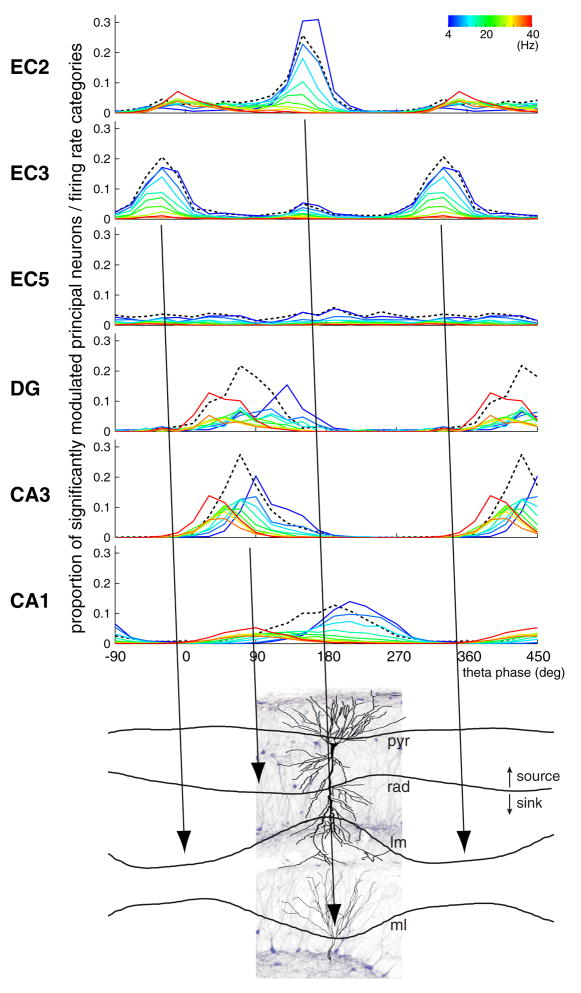
\includegraphics[width=0.70\textwidth]{chapter4/figures/phase-spiking-distributions.jpg}
    \caption{\textbf{Temporal relation between region specific firing patterns}.
    In the top, the histograms reflects the proportion of principal neurons significantly modulated in each firing rate category.
    Dash black line represents the average distribution of the pattern among the categories.
    In the bottom, current source densities for different layers are represented: \textit{str. pyramidale, raditum, lacunosum-moleculare} (CA1) and the \textit{multiforme} or hilus (DG), in a descending way.
    Reversed phases are observed in CA1 \textit{str. lm} and \textit{ml}, along with the shifted phase in \textit{str. rad} when compared to the \textit{lm} sink.
     The arrows show the time differences between the peak firing in preceding layers and the theta sinks in the subsequent layers, reflecting lag of 30º ($\sim$ 10 ms) originated by axonal conduction velocity.
     Original figure from \citep{mizuseki_theta_2009}.}
    \label{fig:phase-spike-distribution}
\end{figure}
This measurement has limitations, particularly when categorizing neurons within the same rate despite differing spike patterns.
For example, neurons firing twice in one cycle and remaining silent in the next are grouped similarly to those firing once in each cycle, both denoted as 8 Hz (blue line). 
Predominantly, neurons categorized at 4 Hz constitute the primary group in each region, with the exception of the Dentate Gyrus principal neurons where bursts (> 40 Hz) hold an equally significant presence alongside those at 4 Hz.

Consequently, our external excitatory inputs were structured around artificial neuron populations from Entorhinal Cortex layers II and III firing at 8 Hz, and two distinct populations within the DG: one representing burst firing and the other firing at 8 Hz.
Choosing 8 Hz over the dominant 4 Hz aimed to simulate neurons firing once every two cycles rather than once per cycle with reduced connectivity, ensuring simulation equivalency and simplicity.

Figure \ref{fig:phase-spike-distribution} guided the use of Gaussian distributions to approximate the spiking pattern distributions.
Each excitatory input group comprised 1000 artificial neurons, following Gaussian distributions aligning with their peak activation times within the cycle.
However, the bursting DG subpopulation varied in that each neuron emitted 5 or 6 spikes per burst, randomly initiated by a Gaussian distribution for the first spike.
Subsequent spikes were generated using a Poisson distribution, ensuring reduced interspike intervals \citep{neubrandt_single_2018}.
The choice of 1000 neurons was determined in order to avoid correlated responses in pyramidal neurons.

The inhibitory neuron population in the Medial Septum consisted of two subpopulations exhibiting out-of-phase dynamics, each containing 10 artificial neurons projecting to basket cells and OLM, respectively \citep{borhegyi_phase_2004}, aligning with previous network models \citep{cutsuridis_computational_2015}.
These neurons fired once per theta cycle.

Table \ref{table:inputs_neurons_synaptic_parameters} details synaptic parameters associated with the external synthetic inputs. 
% \begin{table}[htp]
% \caption{Synpatic parameters in the network: External inputs.}
% \def\arraystretch{1.4}%  1 is the default, change whatever you need
% \begin{center}
%     \begin{tabular}{|c|c|c|c|c|c|c|c|c|}
% \clearpage
% \newpage
\begin{landscape}
\begin{table}[!htb]
\renewcommand\thetable{6} 
\def\arraystretch{1.1}%  1 is the default, change whatever you need
\caption{Synpatic parameters in the network: external inputs.}
\begin{tabular}{|c|>{\centering}p{2cm}|>{\centering}p{2cm}|>{\centering}p{1.4cm}|>{\centering}p{1.4cm}|>{\centering}p{1.4cm}|>{\centering}p{1.4cm}|>{\centering}p{1.4cm}|>{\centering\arraybackslash}p{1.4cm}|}
        \hline
        & Presynaptic & Postsynaptic  & Section & Receptor &$\tau_r$ [$ms$] & $\tau_d$ [$ms$] & $g$ [$nS$] & nproy\\ \hline
         \multirow{18}{*}{\STAB{\rotatebox[origin=c]{90}{External inputs in CA3}}} 
         
         & \multirow{4}{*}{ECII-180} & \multirow{2}{*}{Pyramidal} & \multirow{2}{*}{Adend3} & AMPA & 0.05 & 5.3 & 0.33  & 25 \\ \cline{5-9}
         &                           &                            &                         & NMDA & 15   & 150 & 0.18  & 25 \\ \cline{3-9}
         &                           & \multirow{2}{*}{Basket}    & \multirow{2}{*}{soma}   & AMPA & 0.05 & 5.3 & 0.33  & 25 \\ \cline{5-9}
         &                           &                            &                         & NMDA & 15   & 150 & 0.18  & 25 \\ \cline{2-9}
         & \multirow{4}{*}{ECII-360} & \multirow{2}{*}{Pyramidal} & \multirow{2}{*}{Adend3} & AMPA & 0.05 & 5.3 & 0.0   & 25 \\ \cline{5-9}
         &                           &                            &                         & NMDA & 15   & 150 & 0.0   & 25 \\ \cline{3-9}
         &                           & \multirow{2}{*}{Basket}    & \multirow{2}{*}{soma}   & AMPA & 0.05 & 5.3 & 0.0   & 25 \\ \cline{5-9}
         &                           &                            &                         & NMDA & 15   & 150 & 0.0   & 25 \\ \cline{2-9}
         & \multirow{4}{*}{DG}       & \multirow{2}{*}{Pyramidal} & \multirow{2}{*}{Adend1} & AMPA & 0.05 & 5.3 & 0.09  & 25 \\ \cline{5-9}
         &                           &                            &                         & NMDA & 15   & 150 & 0.05  & 25 \\ \cline{3-9}
         &                           & \multirow{2}{*}{Basket}    & \multirow{2}{*}{soma}   & AMPA & 0.05 & 5.3 & 0.09  & 25 \\ \cline{5-9}
         &                           &                            &                         & NMDA & 15   & 150 & 0.05  & 25 \\ \cline{2-9}
         & \multirow{4}{*}{DG burst} & \multirow{2}{*}{Pyramidal} & \multirow{2}{*}{Adend1} & AMPA & 0.05 & 5.3 & 0.018 & 10 \\ \cline{5-9}
         &                           &                            &                         & NMDA & 15   & 150 & 0.01  & 10 \\ \cline{3-9}
         &                           & \multirow{2}{*}{Basket}    & \multirow{2}{*}{soma}   & AMPA & 0.05 & 5.3 & 0.018 & 10 \\ \cline{5-9}
         &                           &                            &                         & NMDA & 15   & 150 & 0.01  & 10 \\ \cline{2-9}
         & MS-180                    & Basket                     & soma                    & GABA$_\text{A}$ & 0.07 & 9.1 & 0.64 & 10 \\ \cline{2-9}
         & MS-360                    & OLM                        & soma                    & GABA$_\text{A}$ & 0.07 & 9.1 & 0.32 & 10 \\ \hline
       \end{tabular}
\end{table}
\end{landscape}
\begin{landscape}
\begin{table}[!htb]
\ContinuedFloat % To indicate continuation of the previous table
\def\arraystretch{1.1}%  1 is the default, change whatever you need
\caption{Synpatic parameters in the network: external inputs (continuation).}
\begin{tabular}{|c|>{\centering}p{2cm}|>{\centering}p{2cm}|>{\centering}p{1.4cm}|>{\centering}p{1.4cm}|>{\centering}p{1.4cm}|>{\centering}p{1.4cm}|>{\centering}p{1.4cm}|>{\centering\arraybackslash}p{1.4cm}|}
        \hline
        \multirow{11}{*}{\STAB{\rotatebox[origin=c]{90}{External inputs in CA1}}} 
        & \multirow{4}{*}{ECIII-180} & \multirow{2}{*}{Pyramidal} & \multirow{2}{*}{Adend3} & AMPA & 0.05 & 5.3 & 0.0   & 25 \\ \cline{5-9}
        &                            &                            &                         & NMDA & 15   & 150 & 0.0   & 25 \\ \cline{3-9}
        &                            & \multirow{2}{*}{Basket}    & \multirow{2}{*}{soma}   & AMPA & 0.05 & 5.3 & 0.0   & 25 \\ \cline{5-9}
        &                            &                            &                         & NMDA & 15   & 150 & 0.0   & 25 \\ \cline{2-9}
        & \multirow{4}{*}{ECIII-360} & \multirow{2}{*}{Pyramidal} & \multirow{2}{*}{Adend3} & AMPA & 0.05 & 5.3 & 0.33  & 25 \\ \cline{5-9}
        &                            &                            &                         & NMDA & 15   & 150 & 0.18  & 25 \\ \cline{3-9}
        &                            & \multirow{2}{*}{Basket}    & \multirow{2}{*}{soma}   & AMPA & 0.05 & 5.3 & 0.165 & 25 \\ \cline{5-9}
        &                            &                            &                         & NMDA & 15   & 150 & 0.09  & 25 \\ \cline{2-9}
        & \multirow{2}{*}{MS-180}    & Basket                     & soma                    & GABA$_\text{A}$ & 0.07 & 9.1 & 0.64 & 10 \\ \cline{3-9}
        &                            & CCK                        & soma                    & GABA$_\text{A}$ & 0.07 & 9.1 & 0.32 & 10  \\ \cline{2-9}
        &  MS-360                    & OLM                        & soma                    & GABA$_\text{A}$ & 0.07 & 9.1 & 0.32 & 10 \\ \hline
    \end{tabular}
    \label{table:inputs_neurons_synaptic_parameters}
\end{table}
\end{landscape}
In addition, each neuron receives fast excitatory and inhibitory inputs stemming from a background activity created by a Poissonian process operating at a rate of 10 kHz. 
This background noise, simulated as an ongoing stochastic process, provides a continuous influx of excitatory and inhibitory inputs, influencing the membrane potential dynamics of the neurons. The parameters linked to this background activity are detailed in Table \ref{table:background_activity}.
\begin{table}[!htb]
\caption{Parameters of the background activity.}
\def\arraystretch{1.3}%  1 is the default, change whatever you need
\begin{center}
    \begin{tabular}{|c|c|c|c|c|c|c|}
        \hline
        & Neuron & Section & Receptor &$\tau_r$ [$ms$] & $\tau_d$ [$ms$] & $g$ [$nS$] \\ \hline
         \multirow{8}{*}{\STAB{\rotatebox[origin=c]{90}{CA3}}} 
         & \multirow{4}{*}{Pyramidal} & \multirow{2}{*}{Adend3}   & AMPA            & 0.05 & 5.3 & 0.1     \\ \cline{4-7}
         &                            &                           & GABA$_\text{A}$ & 0.07 & 9.1 & 0.012   \\ \cline{3-7}
         &                            & \multirow{2}{*}{soma}     & AMPA            & 0.05 & 5.3 & 0.05    \\ \cline{4-7}
         &                            &                           & GABA$_\text{A}$ & 0.07 & 9.1 & 0.012   \\ \cline{2-7}
         & \multirow{2}{*}{Basket}    & \multirow{2}{*}{soma}     & AMPA            & 0.05 & 5.3 & 0.02    \\ \cline{4-7}
         &                            &                           & GABA$_\text{A}$ & 0.07 & 9.1 & 0.2     \\ \cline{2-7}
         & \multirow{2}{*}{OLM}       & \multirow{2}{*}{soma}     & AMPA            & 0.05 & 5.3 & 0.0625  \\ \cline{4-7}
         &                            &                           & GABA$_\text{A}$ & 0.07 & 9.1 & 0.2     \\ \hline
         \multirow{8}{*}{\STAB{\rotatebox[origin=c]{90}{CA1}}} 
         & \multirow{4}{*}{Pyramidal} & \multirow{2}{*}{Adend3}   & AMPA            & 0.05 & 5.3 & 0.012  \\ \cline{4-7}
         &                            &                           & GABA$_\text{A}$ & 0.07 & 9.1 & 0.012  \\ \cline{3-7}
         &                            & \multirow{2}{*}{soma}     & AMPA            & 0.05 & 5.3 & 0.075  \\ \cline{4-7}
         &                            &                           & GABA$_\text{A}$ & 0.07 & 9.1 & 0.012  \\ \cline{2-7}
         & \multirow{2}{*}{Basket}    & \multirow{2}{*}{soma}     & AMPA            & 0.05 & 5.3 & 0.012  \\ \cline{4-7}
         &                            &                           & GABA$_\text{A}$ & 0.07 & 9.1 & 0.2    \\ \cline{2-7}
         & \multirow{2}{*}{OLM}       & \multirow{2}{*}{soma}     & AMPA            & 0.05 & 5.3 & 0.0625 \\ \cline{4-7}
         &                            &                           & GABA$_\text{A}$ & 0.07 & 9.1 & 0.2    \\ \cline{2-7}
         & \multirow{2}{*}{CCK}       & \multirow{2}{*}{soma}     & AMPA            & 0.05 & 5.3 & 0.045  \\ \cline{4-7}
         &                            &                           & GABA$_\text{A}$ & 0.07 & 9.1 & 0.012  \\ \hline
    \end{tabular}
    \label{table:background_activity}
\end{center}
\end{table}

\subsubsection{Output of the network}
The network model encompasses various outputs recorded from each neuron, including \textbf{spikes} and \textbf{membrane potentials}, with a detailed focus on the membrane potential of individual compartments in pyramidal cells.
Additionally, synaptic currents received by each compartment of pyramidal cells were recorded.
% A collective measurement, the \textbf{Local Field Potential} (LFP), was computed considering the \textbf{line source approximation} given by \eqref{eq:line-source-approximation}.
% This computation involves a summation of contributions from each compartment of pyramidal neurons (in CA3 or CA1), referencing the electrode's position.
The \textbf{Local Field Potential} (LFP) primarily reflects synaptic activity in nearby neural ensembles, with dendritic synapses on pyramidal cells hypothesized to be a major contributor \citep{linden011859,https://doi.org/10.1113/JP279452}.
Therefore, for the LFP computation, we considered the \textbf{line source approximation} (equation \eqref{eq:line-source-approximation}) involving only the contributions from the compartments of each pyramidal neurons (in CA3 or CA1).
For simplicity, we organized the pyramidal cells of CA3 and CA1 subfields into a rectangular grid with a 50 $\mu$m separation, aligned parallel to the $z$-axis.
In this configuration, the center positions of each (CA3 or CA1) pyramidal cell compartment were designated as -100, 10, 85, 235, and 385 $\mu$m for Bdend, soma, Adend1, Adend2, and Adend3, respectively.
We positioned five electrodes for simulations at the center of the grid, each aligned parallel to a specific compartment of pyramidal cells.
This arrangement aimed to facilitate the measurement of five distinct LFP references across different layers within our network model.
An example of the resultant LFPs in the network model is shown in Figure \ref{fig:LFP-example}.
\begin{figure}[!htb]
    \centering
    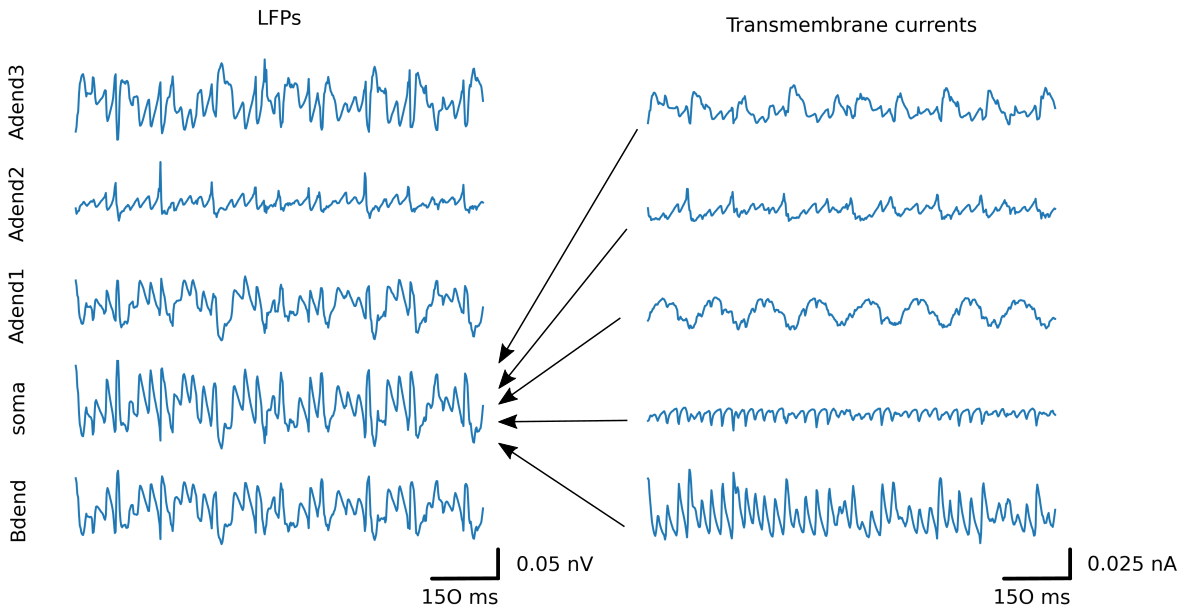
\includegraphics[width=\textwidth]{chapter4/figures/LFPs.png}
    \caption{\textbf{Local field potentials}. 
    The right panel displays five distinct LFPs recorded from each layer of the CA3 subfield.
    Electrodes are positioned along the $z$-axis at the center of each compartment of the pyramidal cells.
    The left panel illustrates the transmembrane currents of each layer from which the LFP is computed.}
    \label{fig:LFP-example}
\end{figure}

On the other hand, the finite-size constraint impacts the dynamic of the network model, suggesting an inclination toward larger neuron populations for improved accuracy.
To investigate this, we designed a network of pyramidal cells organized in a rectangular grid with a 50 $\mu$m separation, each stimulated by excitatory noise inputs at both the soma and the most distal dendrite.
Figure \ref{fig:finite_size_effect} B shows the evolution of the average LFP amplitude as the number of pyramidal cells increases.
While the mean of the LFP increases monotonically, the amplitude rapidly reaches a plateau.
Increasing the number of neurons could potentially improve the precision of the metrics used, however, this may not lead to a proportional increase in magnitude, as the amplitude remains relatively constant.
Figure \ref{fig:finite_size_effect} C illustrates the variation of the average amplitude of LFP with the distance to the center.
As expected, the LFP amplitude reaches its maximum at the center of the network.
\begin{figure}[!htb]
    \centering
    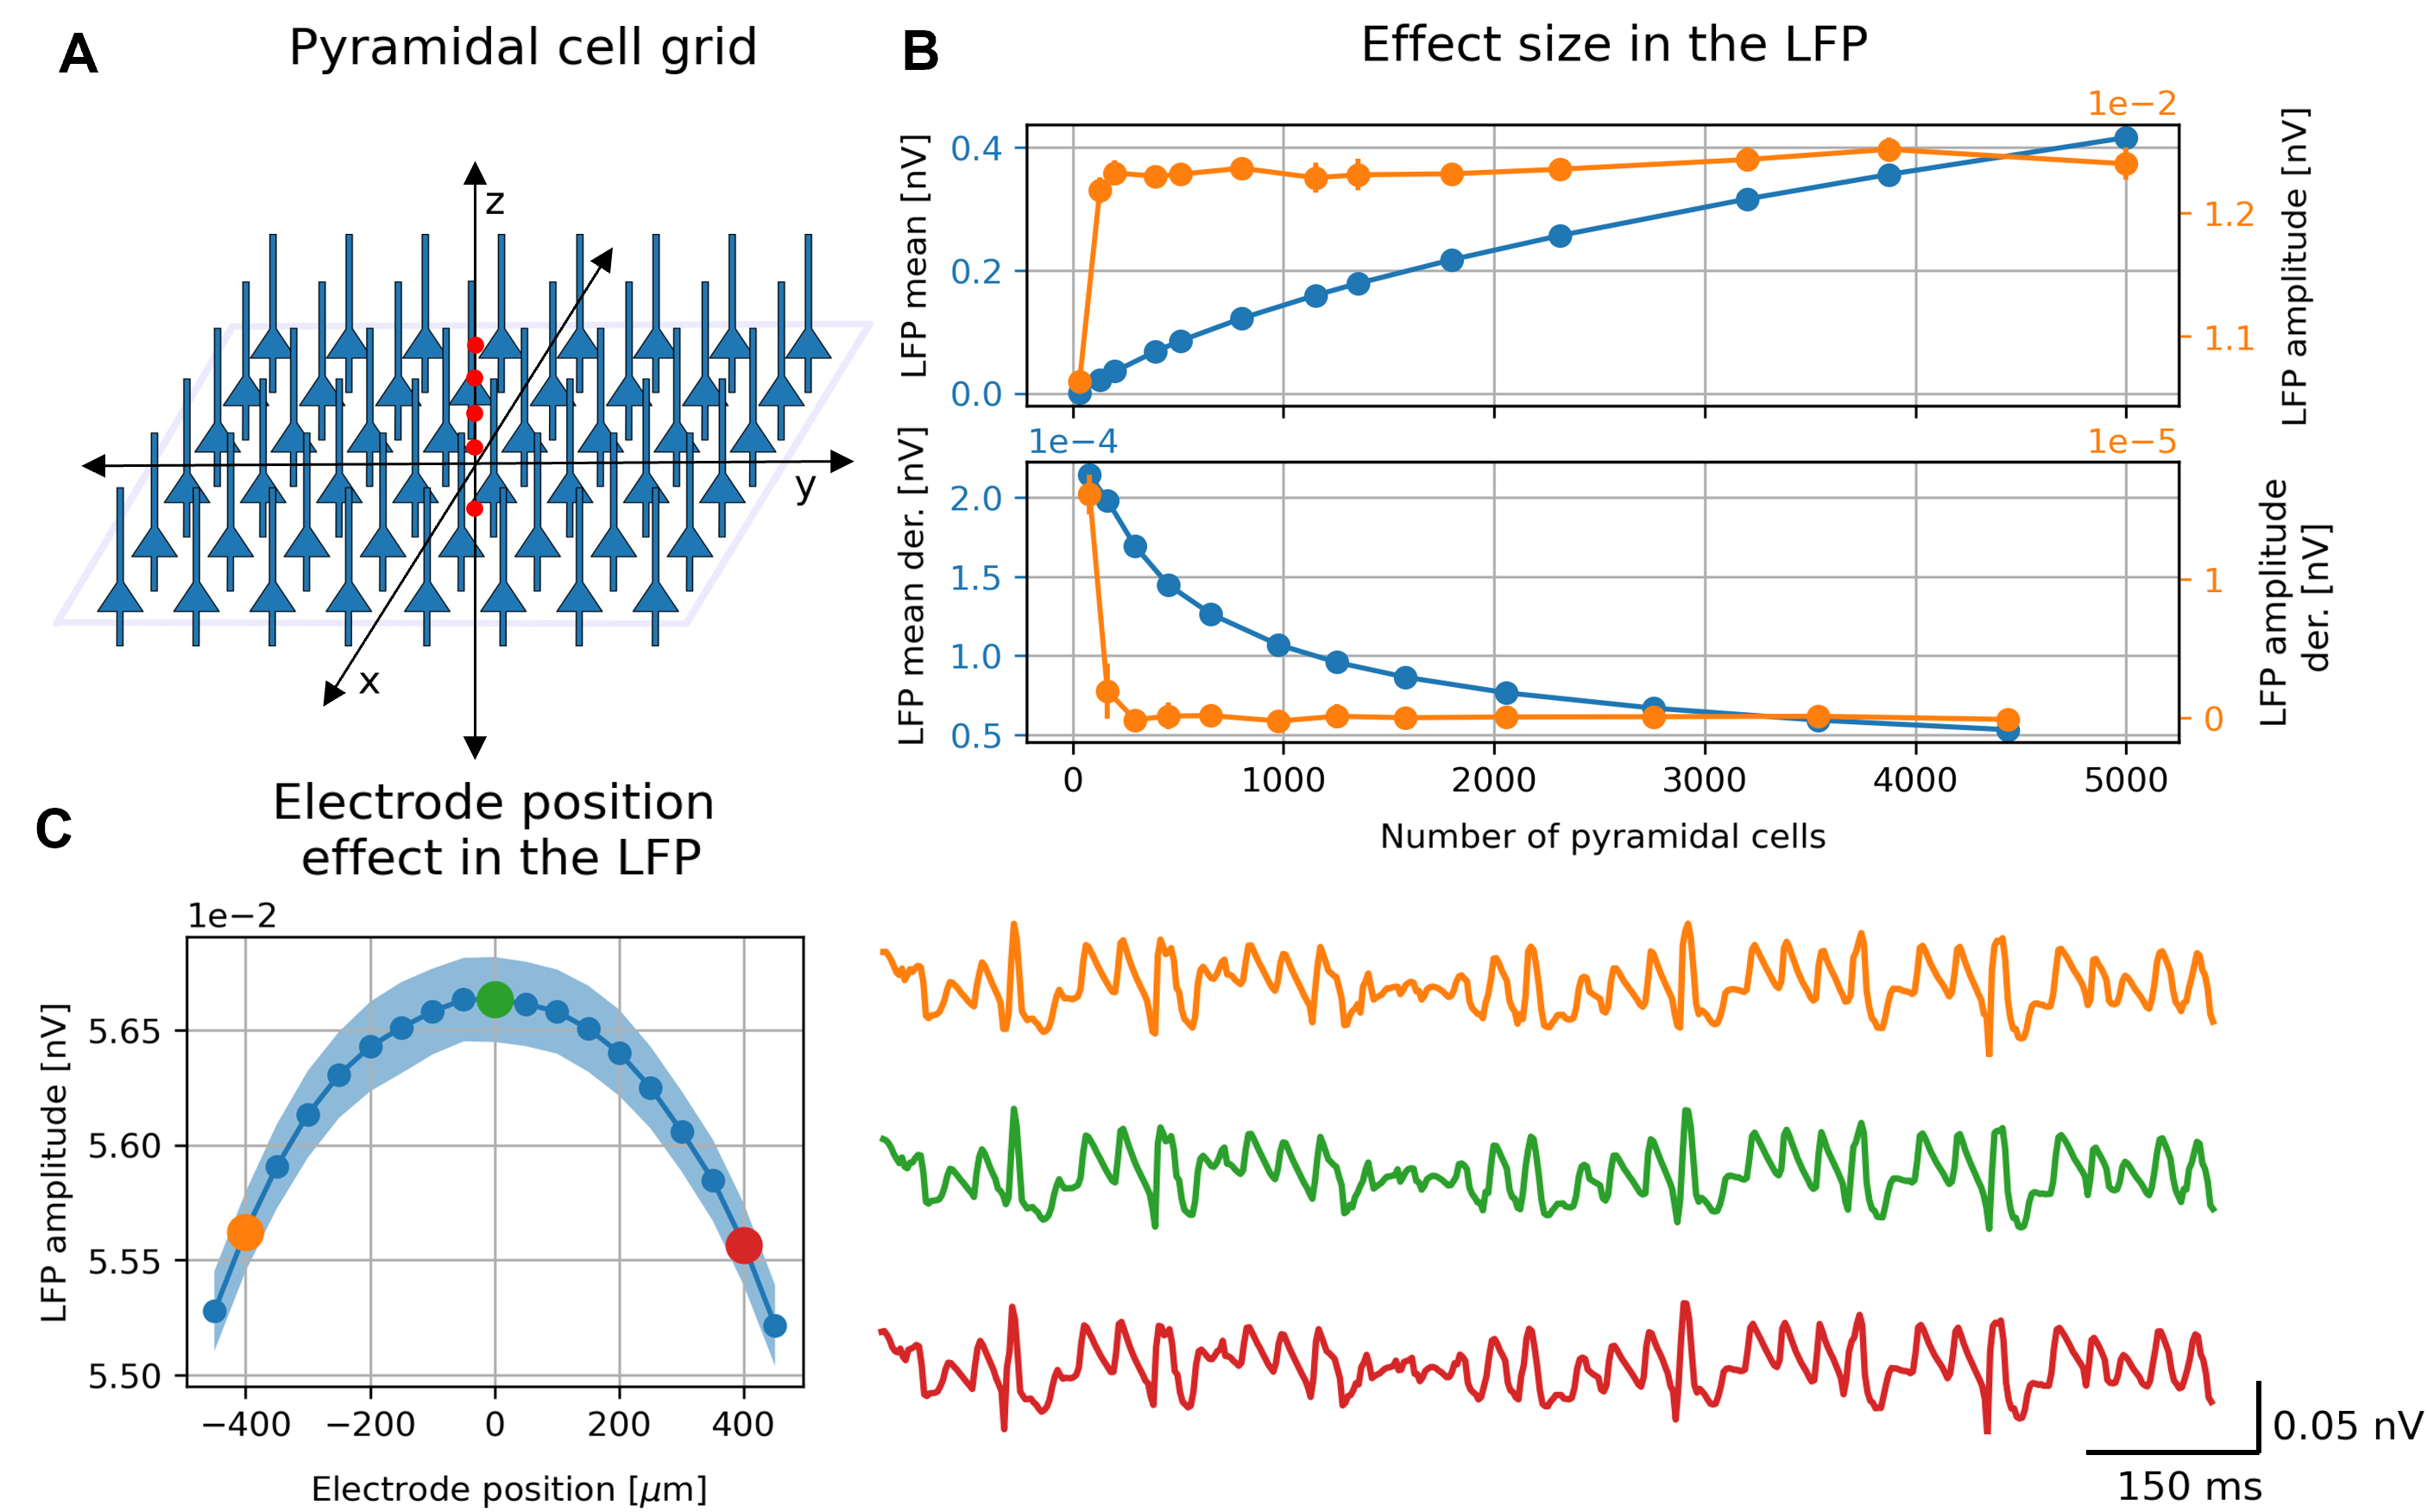
\includegraphics[width=\textwidth]{chapter4/figures/LFPproperties.png}
    \caption{\textbf{Finite-size network effect in the LFPs}.
    Panel A illustrates the poistioning of pyramical cells in the network with the electrodes placed alongside the $z$-axis. 
    Panel B shows the variation of the mean and amplitude (and their derivatives) of the LFP in a grid composed of interconnected pyramidal neurons.
    Panel C shows the variation of the soma LFP amplitude as the electrode position changes respect to the center of the grid.
    The amplitude is measured as twice the standard deviation of each signal of the soma measured at the correspondent position.
    Shadowed band colour
    indicates the error.
    The three different points indicate the examples of the LFP shown in the right side.}
    \label{fig:finite_size_effect}
\end{figure}
% \begin{figure}
%     \centering
%     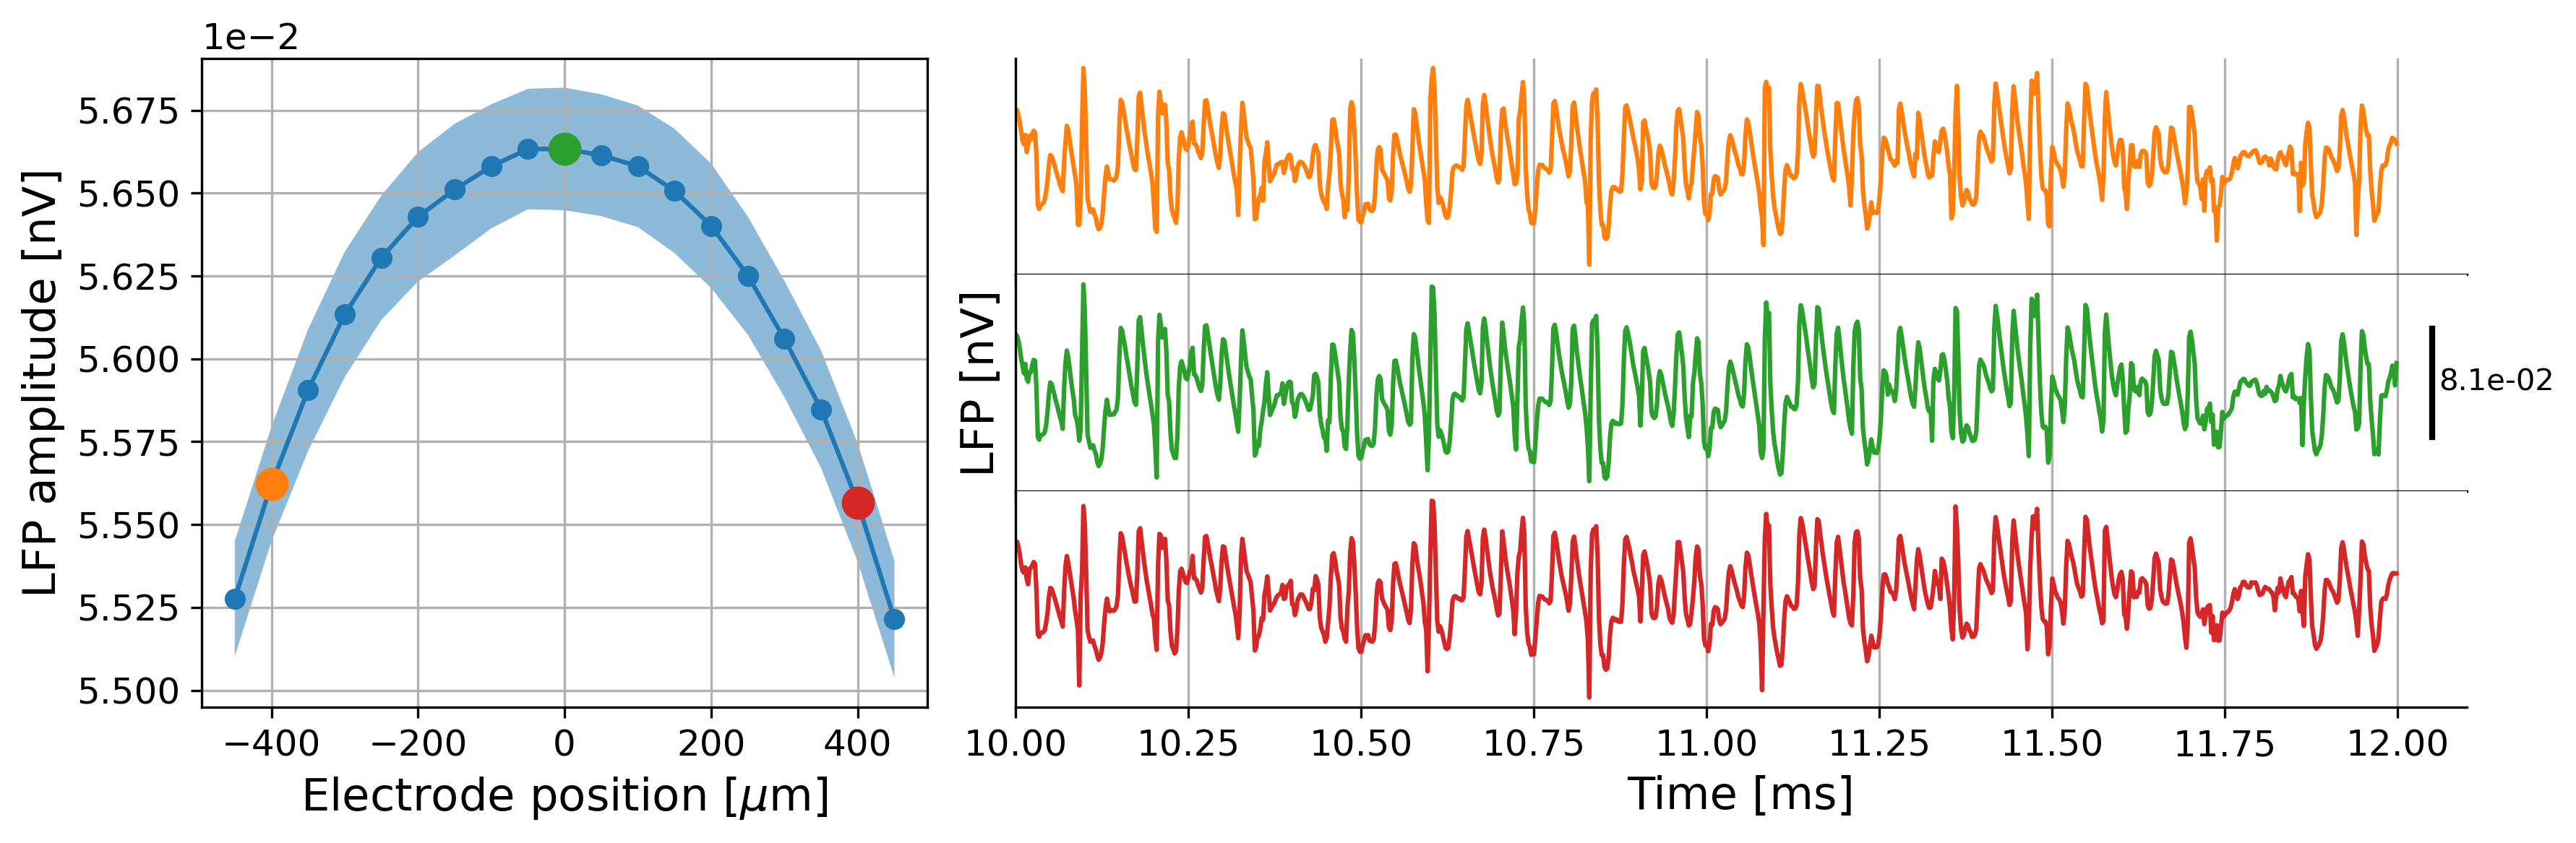
\includegraphics[width=\textwidth]{chapter4/figures/electrode_position.png}
%     \caption{Variation of the soma LFP amplitude as the electrode position changes respect to the center of the grid.
%     The amplitude is measured as twice the standard deviation of each LFP signal of the soma measured at the correspondent position.
%     Shadowed band colour indicates the error.
%     The three different points indicate the examples of the LFP shown in the left panels. }
%     \label{fig:LFP_amplitude_distance}
% \end{figure}
\subsection{Measuring phase-amplitude coupling} 
Over the past two decades, numerous metrics have emerged to quantify phase-amplitude cross-correlation, many of which rely on extracting the instantaneous phase and amplitude of band-pass-filtered signals via the Hilbert transform.
Among the most widely used measurements for phase-amplitude coupling are the phase-locking value (PLV) \citep{mormann_phaseamplitude_2005, cohen_assessing_2008}, mean vector length (MLV) \citep{canolty_high_2006}, modulation index (MI) \citep{tort_dynamic_2008}, generalized linear modeling method (GLM) \citep{kramer_assessment_2013}, phase binning combined with analysis of variance (BA) \citep{lakatos_oscillatory_2005}, weighted phase locking value (wPLV) \citep{maris_spatially_2011}, and mutual information \citep{martinez-cancino_measuring_2019}.

While PLV effectively captures phase synchronization between signals, it may not consistently represent amplitude modulation accurately.
In contrast, methods such as GLM and MLV offer a deeper understanding of the phase-amplitude relationship, albeit with increased computational complexity and potential assumptions regarding the underlying data distributions.
The Modulation Index (MI) is particularly notable for its capacity to quantify high-frequency oscillation amplitude modulation by a low-frequency oscillation phase.
In particular, MI exhibits robustness in capturing cross-frequency coupling phenomena and demands lower computational resources compared to other methods.
The versatility and reliability of this method in capturing phase-amplitude interactions have been demonstrated across diverse neuronal datasets, further solidifying its utility in research and analysis \citep{caixeta2013ketamine,fernandez-ruiz_entorhinal-ca3_2017,fernandez2021gamma,lopez-madrona_different_2020}.
\subsubsection{Modulation index}
Following the analysis done by Lopez-Madrona \textit{et al.} \citep{lopez-madrona_different_2020}, we adopted the \textbf{Modulation Index} (MI) as a metric to quantify phase-amplitude cross-frequency coupling between theta and gamma oscillations.
To compute the MI for a given time series $x(t)$, such as the LFP, accurate determination of the instantaneous phase of theta oscillations and the amplitude of gamma oscillations is pivotal.
The conventional approach involved band-filtering of the raw signal to extract the theta and gamma components.
Subsequently, employing the Hilbert transform facilitated obtaining the instantaneous phase and the envelope, respectively.
However, theta rhythms in the hippocampus often demonstrate non-sinusoidal oscillations. Filtering such signals may inaccurately estimate waveform shapes and introduce spurious coupling \citep{cole2017brain, kramer2008sharp}.
In response to this concern, a novel methodology was proposed, specifically designed to precisely estimate the instantaneous phase of these oscillations \citep{cole2019cycle}. This innovative approach employs a two-tiered filtering technique: firstly, a narrowband filter identifies zero-crossing points, representing ascending and descending slopes (equivalent to phases $\pi/2$ and $3\pi/2$, respectively).
Subsequently, a broadband filter pinpoints trough and peak phases (0 and $\pi$, respectively).
This method accommodates rapid alterations within the cycle, preserving the non-monotonic phase changes inherent in non-sinusoidal oscillations.

Determining the amplitude of the faster oscillation involves computing the envelope of the signal filtered at the specific frequency band under analysis.
We applied a filter centered at the target frequency, ensuring a bandwidth at least twice the frequency of the phase signal to optimize capturing maximal coupling \citep{aru2015untangling}.
In our analysis, due to 8 Hz is the primary rhythm, a minimum bandwidth of 16 Hz was necessary.
Subsequently, applying the Hilbert transform to this filtered signal enabled the extraction of the envelope, resulting in the signal denoted as $x^{\gamma}_A(t)$.

For the MI computation, we segmented each cycle of phase of the theta-filtered signal $x^{\theta}_{\varphi}$ into $N$ bins. 
Using the two-tiered technique, these $N$ bins were equal along the phase of the cycle, rather than equal in time.
Each cycle was divided into 4 segments, corresponding to epochs between the peak, trough, and both ascending and descending slopes.
Further, these segments were divided into $N/4$ bins of the same size. Consequently, $N/4$ bins were utilized from the trough to the middle of the ascending phase, $N/4$ bins from this point to the peak, and so forth.
Alternatively, with the traditional method, the binning resulted in equal time and phase bins, obtained by segmentation from trough to peak.
Subsequently, we computed the mean amplitude of $x^{\gamma}_A(t)$ at each bin, denoted as $\langle x^{\gamma}_A\rangle_{j}$, representing the amplitude at phase bin $j$. 
From these values, we derived the entropy $H$, defined by:
\begin{equation}
    H = -\displaystyle\sum_{j=1}^{N}p_j \log p_j,\\
    \label{eq:entropy}
\end{equation}
where $N$ was set to 20 bins, and the distribution $p_j$ is given by: 
\begin{equation}
    p_j = \displaystyle\frac{\langle x^{\gamma}_A \rangle_{\varphi,j}}{\displaystyle\sum_{k=1}^{N}\langle x^{\gamma}_A \rangle_{\varphi,j}}.
    \label{eq:amplitude-probability}
\end{equation}
The value of MI is defined as the entropy $H$ normalized by the maximal entropy $H_\text{max}$ ($\log N$), given by:
\clearpage
\begin{equation}
    MI = \displaystyle\frac{H_\text{max}-H}{H_\text{max}}.
    \label{eq:modulation-index}
\end{equation}
A value of MI near 0 indicates lack of phase-to-amplitude modulation, while larger MI values reflect higher coupling between both signals.

We implemented both methodologies, phase extraction via the Hilbert transform and the two-tiered filtering technique.
Despite the differences in the instantaneous phase estimations between these methods, our analysis revealed negligible differences in the resulting MI.
Given the comparable outcomes observed in MI calculations, and considering computational efficiency, we made a deliberate choice to adopt the traditional Hilbert transform method.

%%%%

% \printbibliography
\end{document}
% \subsection*{Welch's method}
% The Welch's method \citep{welch_use_1967} is an approach of spectral density stimation. This method consists in two steps. First, the signal x(t) is split up into $k$ overlapping segments $\{x(t)_s\}_{s=1}^{k}$ of the same length $L$. Then, the segments are windowed, for example using the Hamming window $\{h(t)\}_{s=1}^{k}$.  
% Finally, the periodogram is calculated by compute the square value of the discrete Fourier transform $\{ X(f)_s\}_{s=1}^{k}$. Computationally, the fast Fourier transform algorythm is more efficient when the dimension of each segment is a power of two, then zero-padding technique helps not only to increase the efficiency but increase the resolution in the frequency domain citar. This technique constists on adding zeros in the signal until the total length is a power of 2.

about CFC 

In the computation of the MI, the choice of filtering bandwidth results into a pivotal parameter in both detecting and interpreting the cross-frequency interactions.
The theta and gamma components, obtained post-filtering, are heavily influenced by the chosen center frequencies and the bandwidth surrounding them.
Common practice involves scanning a range of center frequencies for both phase and amplitude components within a narrow bandwidth of a few Hz.
However, the chosen bandwidth plays a critical role in defining what is identified as a component and how its power evolves over time.
For instance, contrasting effects will be observed if frequency scans are conducted from 20 Hz to 60 Hz with a bandwidth of 2 Hz, as opposed to employing a single filter centered at 40 Hz with a broader bandwidth of 21 Hz.
While the bandwidth for the phase (theta) component is often rightly selected to be narrow, ensuring precise characterization of phase dynamics, the amplitude component demands a more meticulous selection of bandwidth.
This includes accounting for the side peaks engendered by the lower frequency, failing which, the presence of CFC could be overlooked, leading to false negative results.
It is mandatory that the bandwidth of the amplitude component is at least equal to twice the modulation frequency to accurately capture and represent the CFC dynamics.
This intricate interplay between bandwidth selection and accurate computation of the MI underscores the nuanced approach necessary for a reliable and meaningful analysis of cross-frequency coupling in neuronal data \citep{aru_untangling_2015}.

To test statistical significance of this metric, a surrogate analysis has been assessed (n=1000) in which each surrogate is built by cutting the gamma envelope signal at different random points and shuffling the resultant segments.
Therefore, the MI values of all surrogates are approximated to a gaussian distribution and the percentile was set to 95\%.
